 \section{Methodology}\label{sec:methodology}
We analyzed BGP RIB data from April 2017 and classified instances where we saw multiple ASes announcing the same BGP prefix. We analyzed the BGPStream data from the first hour of every day in the hopes of identifying hijacks, misconfigurations and other reasons for origin-AS conflicts. The known BGP hijacks of this time were [..... list a few hijacks]which our method successfully  identifies. \\
The goal of this study was to understand the frequency and the duration of censorship intended or malicious BGP hijacks. In addition, we  use our data and our understanding of current socio-political situation surrounding the hijack to understand the popular motives behind BGP hijacks. Towards the end, based on our analysis of how most of the hijacks were accomplished, we recommend possible solutions to prevent accidental and malicious BGP hijacks. 
There is a visualization of the following protocol flow in Figure 2.

 \begin{figure}[!htbp]
	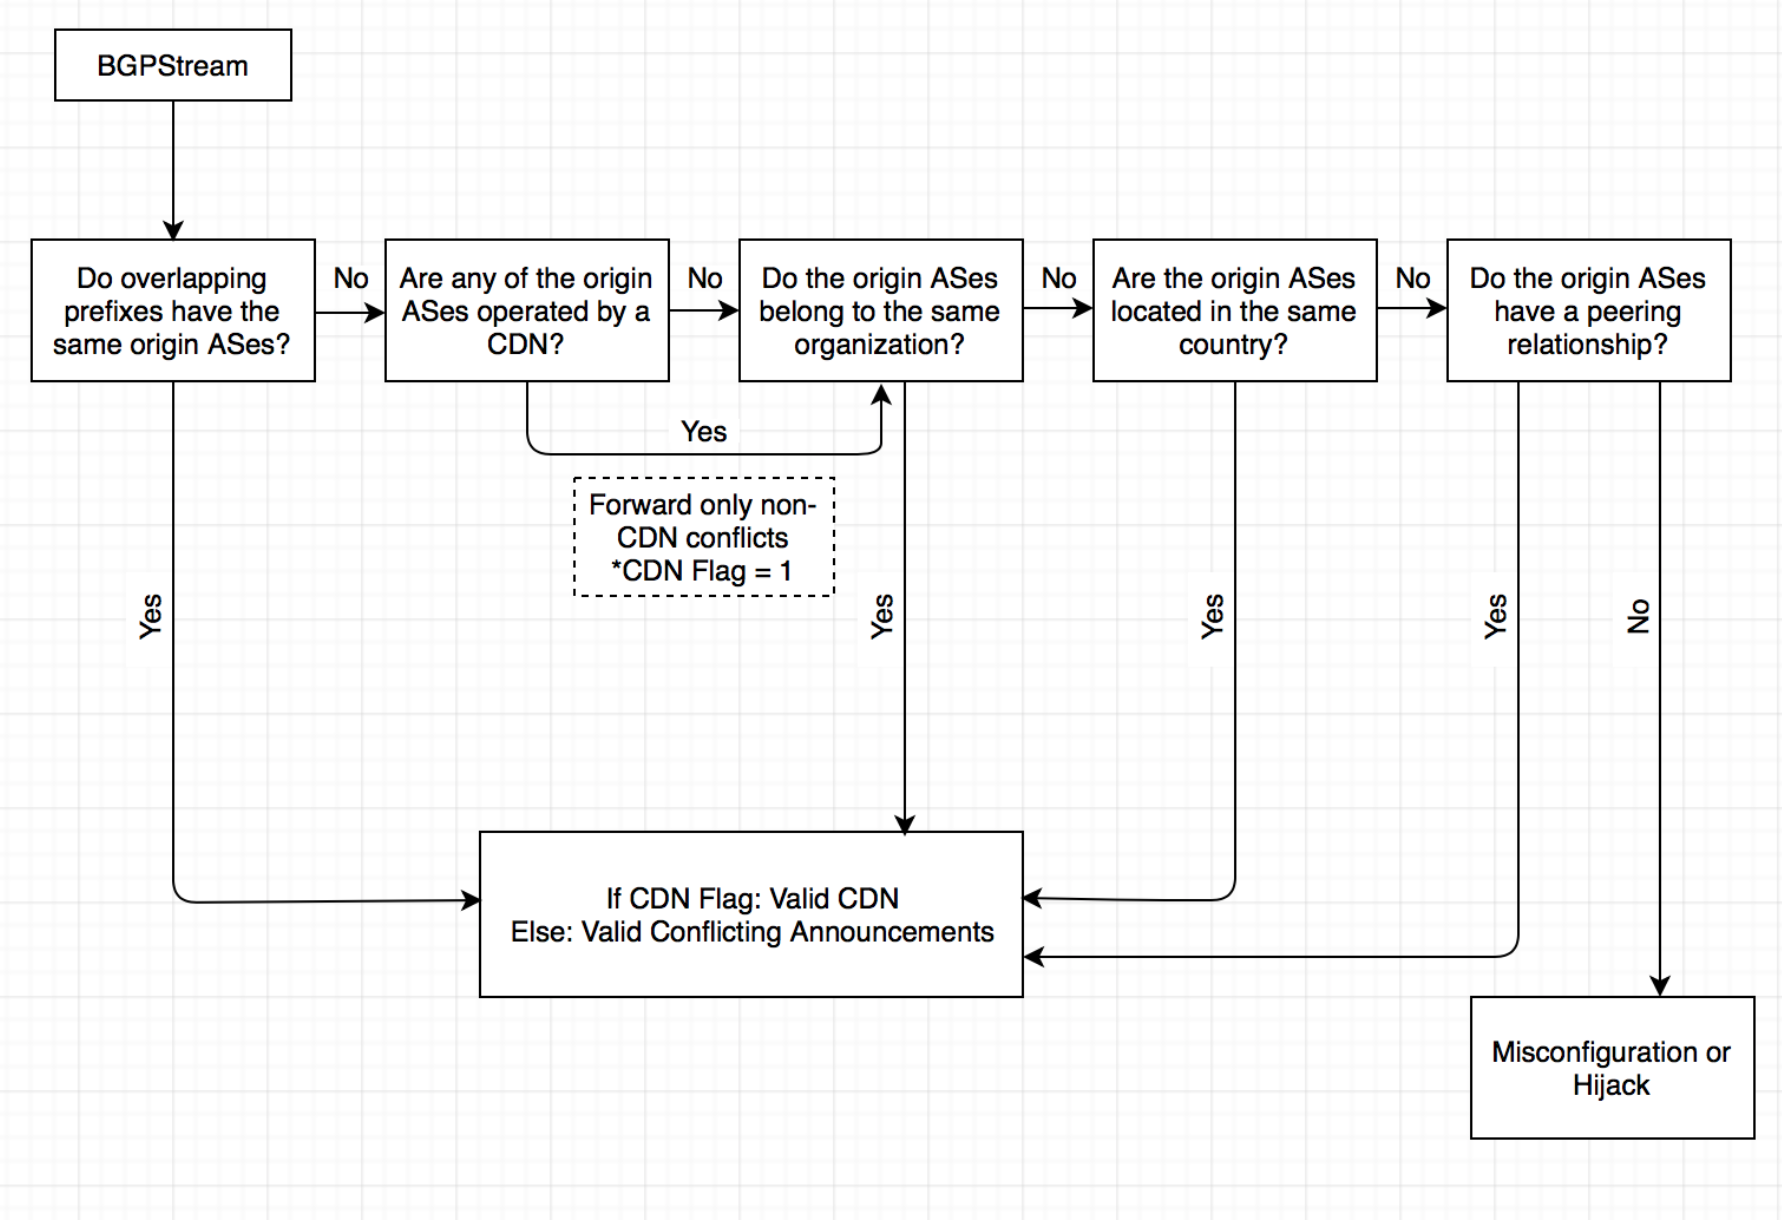
\includegraphics[width=0.5\textwidth]{flow.png}
	\caption{Our algorithm flow chart through which AS-origin conflicts were categorized using BGPStream and CAIDA.}
	\label{a:label}
\end{figure}

\subsection{Identifying Source of Conflict}
Identifying the source of the AS conflict involve a carefully filtering RIB table records. 
\begin{enumerate}
\item The first step is identifying the instances where we saw two different ASes announcing the same BGP prefix/es.
\item We use CAIDA AS information to check if any origin AS owner is a CDN. CDN's may announce the same prefix in different parts of the world for traffic engineering. This lead to clients being directed to the closest CDN cache. If any AS is operated by a CDN, we set a flag, noting the existence of a CDN, and only forward ASes for further filtering which are not a part of it. 
\item We use whois records and the CAISA AS information data  to check if the different ASes belong same organization. If so, we label the conflict as resulting from an international organization.
\item If the ASes do not belong to the same organization, we check the countries of ownership using the same CAIDA dataset as in the previous two steps. If the countries are the same, we consider the conflict to be valid - in other words, not caused by a hijack or misconfiguration.
\item If the ASes annoucing the same prefix do not belong to the same organization or country, we check if they have a peer-to-peer or a customer-provider relationship. We used the CAIDA AS-Relationship dataset to identify these relationships. This idea of using business relationship was inspired by OpenDNS's classification of BGP \cite{opendns_blackhat_2015}. It is likely that ASes with business relationships have permission to announce these conflicting prefix. 
\item If there is no identifiable AS relationship, and the countries and organizations operating the ASes are different, we label the conflict a hijack or a misconfiguration. In order to decide which label to assign to the conflict, we check the prefixes and ASes in question against the BGPStream twitter stream and manually search for information about this conflict.
\end{enumerate}

Based on the sociopolitical context and other information we have [...what other infor? ], we manually classify into three categories (1)Misconfiguration, (2)Political hijack for Censorship and (3)Malicious non-political hijack. 

We enumerate the specificity and the number of malicious BGP prefix announcement for each hijack. We calculate the difference in the specificity of the prefix announced by the hijacking AS and the hijacked AS. To determine if there is a cross-national involvement in these hijacks, we enumerate the number of malicious AS prefix announcement for each hijack. We study the geographic distributions of each of the malicious ASes.
We also characterize the target ASes of these hijacks. We determine whether the target selected (1)randomly/for fun , (2) for financial motive, (3) political motive .
\subsection{Hijack Duration and frequency}

